% First, we share the results for house prices. Next, we present the results for employment and wages outcome variables.

% \subsection{Local government spending}



\subsection{Road Quality decline} \label{sec:road_quality_decline}

 To assess the impact of cutting local road taxes on road quality, we utilized a fine-tuned Vision Transformer (ViT) model, leveraging labeled satellite imagery data for U.S. roads. The ViT model, fine-tuned using a large dataset of road images, assigned quality ratings on a scale of 0 (poor) to 2 (high) to our collected satellite imagery for Ohio neighborhoods, as explained in Section \ref{sec:road_quality}. We compared road quality ratings from the fine-tuned ViT model before and after the referendum in areas that failed to renew their road tax levy versus those that successfully passed the levy. These results are visually summarized in Figure \ref{fig:road_quality_change}, which shows the change in road quality ratings for both groups. 


\begin{figure}[htbp]
    \centering
    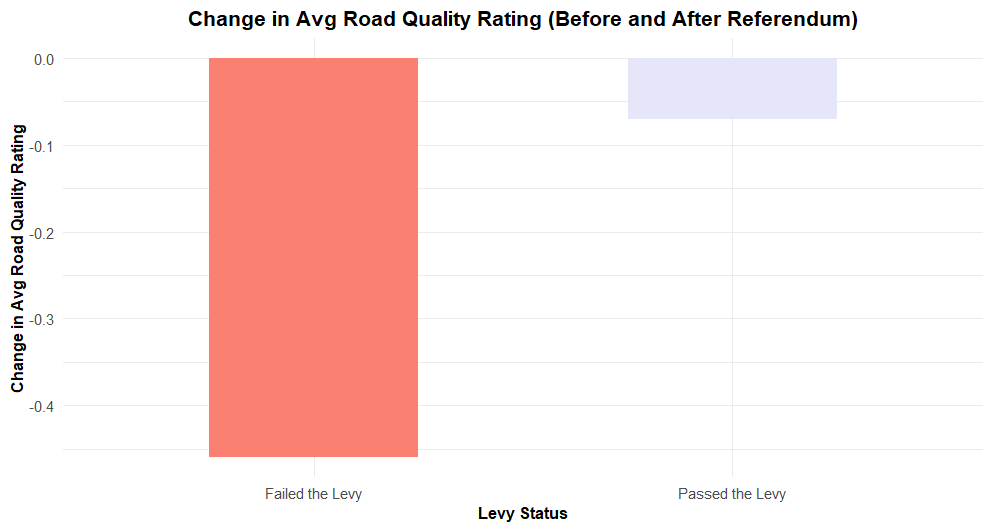
\includegraphics[width=\textwidth,keepaspectratio]{images/road_quality_change.png}
    \caption{Change in Road Quality Ratings Before and After Referendum}
    \label{fig:road_quality_change}
\end{figure}

Areas that failed to renew their tax levy experienced an average decline in road quality ratings of -0.5 points, equivalent to a 17\% deterioration in road quality relative to the three-point scale. In contrast, areas that maintained their tax levies saw a negligible decline of -0.08 points, suggesting effectively no deterioration in road quality. In neighborhoods where renewal taxes were cut, the decline in road quality highlights the potential long-term implications of fiscal policy decisions on public infrastructure maintenance.

\subsection{House Prices decline}

 Table \ref{tab:median_sale_amount} below shows the ITT estimates of failing a road tax levy on housing sale prices starting four years after the vote. 

 \begin{table}[ht]
    \centering
    \caption{Effect on median house prices of failing to renew a road tax levy}
    \label{tab:median_sale_amount}
    \begin{tabular}{p{2cm}ccccccc}
        \hline
        Year relative to vote & $t + 4$ & $t + 5$ & $t + 6$ & $t + 7$ & $t + 8$ & $t + 9$ & $t + 10$ \\
        \hline
        Treatment effect & -21,684 & -22,415 & -17,539 & -16,001 & -21,973 & -19,890 & -16,042 \\
        Standard error   & (7,838) & (8,348) & (8,465) & (6,918) & (9,111) & (7,756) & (8,915) \\
        Effective bandwidth ($h$) & 8.508 & 10.573 & 9.613 & 13.390 & 8.240 & 7.233 & 6.404 \\
        Bias bandwidth ($b$) & 16.430 & 19.894 & 17.133 & 23.953 & 15.327 & 14.073 & 16.469 \\
        Effective Observations & 469 & 605 & 525 & 801 & 402 & 324 & 260 \\
        Total Observations & 2,614 & 2,531 & 2,438 & 2,324 & 2,199 & 2,115 & 2,017 \\
        \hline
    \end{tabular}
    \begin{tablenotes}
        \small
        \item Outcome is median house price in constant 2010 U.S. dollars. Unit of observation is the city-year, so a treatment effect of -\$21,684 means that four years after the vote, cities that failed to renew road taxes and its associated spending have houses that sell for \$21,684 less than cities that vote to renew road taxes and spending. Treatment effects for years prior to $t + 4$ are statistically insignificant at the 5\% level; full results shown in Table \ref{tab:median_sale_amount_full}. The regressions include covariates related to the demographics and socioeconomic factors of the cities, drawn from Table \ref{tab:variable_means_sd}.
    \end{tablenotes}
\end{table}


Each treatment effect estimate represents the discount in median sale price for cities that cut road taxes in the years after voting on a road tax levy relative to otherwise similar cities that renew the taxes. Treatment effect estimates for years 4 through 9 after the vote are statistically significant in Table \ref{tab:median_sale_amount} as the $p$-values are below the canonical 0.05 threshold. The estimate for year $t + 10$ has a smaller estimate and is only significant at the 10\% level, suggesting that the effect of tax and service cuts on house prices may peter out ten years after the vote. Overall, we find an average reduction of \$15,349 in median house price over the 10 year period for houses in cities that vote to cut road tax levies representing 9\% of overall home value.\footnote{The average treatment effect estimate of \$15,349 was divided by the mean home sale price in the dataset of \$166,000 to get 9\%.}

\begin{figure}[htbp]
    \centering
    % 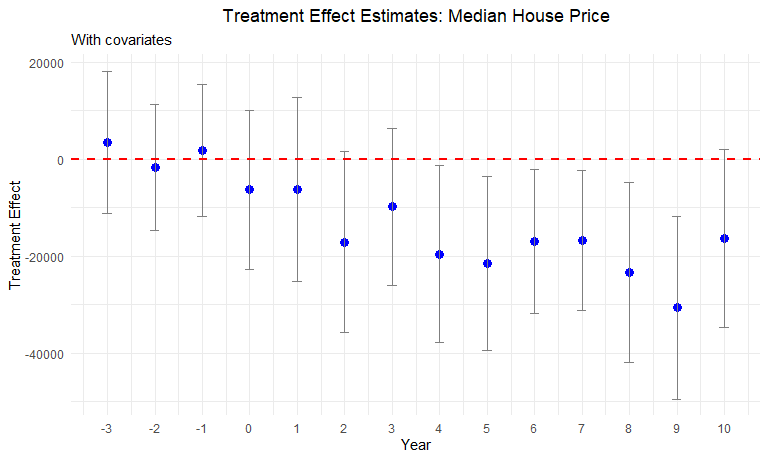
\includegraphics[width=\textwidth,keepaspectratio]{images/tes_gs.png}
    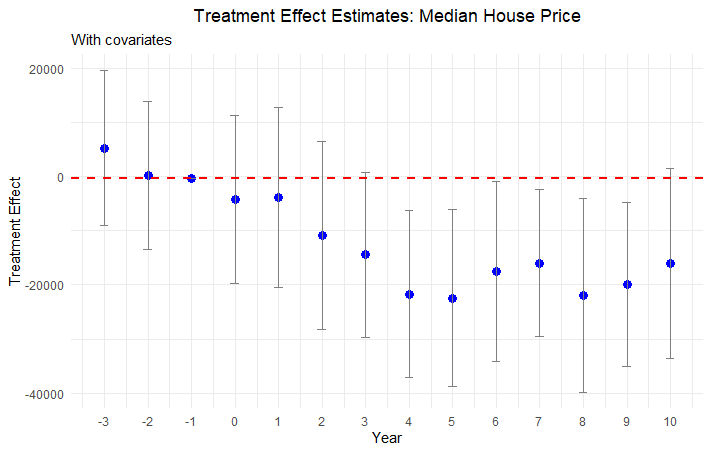
\includegraphics[width=\textwidth,keepaspectratio]{images/tes_gs_reg.png}    
    \caption{Effect plot for Median Housing Price}
    \label{fig:tes_hp}
\end{figure}

Figure \ref{fig:tes_hp} provides an event-study plot that summarizes the treatment effects for each time period. In the graph, we include placebo years up to 3 years before the treatment to show that the median housing prices are statistically identical for cities above and below the threshold prior to the treatment. Each blue dot represents the treatment effect estimate for that year and the bar around it represents the 95\% confidence interval for that estimate. For year 0, which is the year of the vote, we see a slight decrease in the estimate. However, this effect is not statistically significant, as evidenced by the confidence interval containing the null effect. Up to year 3, we observe that the treatment effect estimates are fairly close to zero, and the confidence interval overlaps with zero. As stated previously and shown in Table \ref{tab:median_sale_amount}, we start to see a sizable increase in treatment effect from year 4 onwards and continue to observe it through year 9 after the vote. 
 
\subsection{Heterogeneity Analysis} 

We show the results of our heterogeneity analysis, where we explore the differential impact of cutting road maintenance spending on house prices based on urban vs rural neighborhoods, the size of the tax levy and housing price quantiles.

\vskip 0.5cm

\textbf{Urban vs Rural neighborhoods}: We perform heterogeneity analysis to assess whether different types of neighborhoods and differing size of tax levies result in a differential impact on the housing prices. We first compare urban and rural areas in Ohio. We consider two different ways to define a city as urban:  one including only urbanized areas and another one including both urban areas and urbanized clusters. The event study plot in Figure 6 shows this result. 

\begin{figure}[htbp]
    \centering
    % 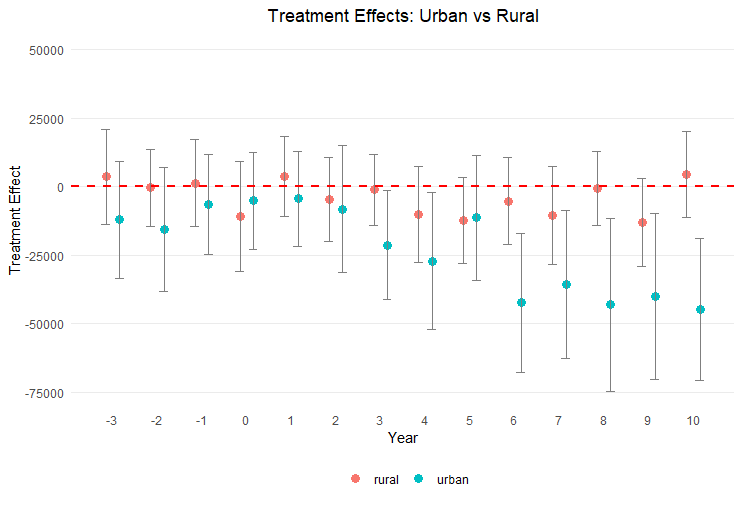
\includegraphics[width=\textwidth,keepaspectratio]{images/tes_covs_ua_new.png}
    % 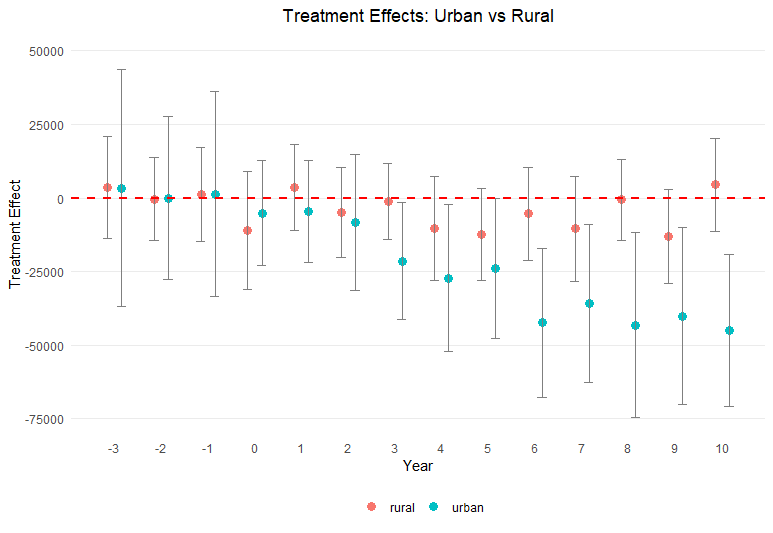
\includegraphics[width=\textwidth,keepaspectratio]{images/tes_covs_ua_clean.png}    
    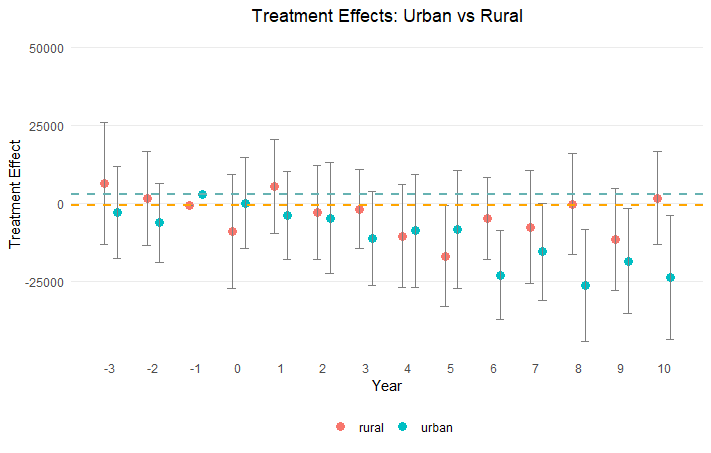
\includegraphics[width=\textwidth,keepaspectratio]{images/tes_covs_ua_reg.png}        
    \caption{Median Housing Price in Urban and Rural Areas}
    \label{fig:tes_covs_ua}
\end{figure}

As shown by Figure \ref{fig:tes_covs_ua}, we do not find any significant differences in housing prices after a renewal tax levy fails to pass for rural areas. On the other hand, we do find a statistically significant decline in housing prices in urban areas starting six years after voting. The standard errors are somewhat smaller for the rural estimates due to a larger number of observations. The difference in point estimates between urban and rural areas may stem from differences in housing supply elasticity (Brasington 2002). Overall, we find that housing prices decrease by \$13,302 on average over the decade\footnote{This is equal to $7.6\% = \frac{13,302}{175,217} \times 100$, where the denominator is average sale price of homes in urban areas in our dataset} after cutting road maintenance tax levies in urban areas. 

\vskip 1cm

\textbf{Tax magnitude}: We check whether the treatment effect is greater for bigger tax levies than smaller tax levies. For this analysis, we split the tax levies based on the millage of a tax levy that is voted upon, where one mill is one tenth of one percent. Mean millage in our dataset is 1.9. We split the data into two parts: small tax levies $\le$ 1.9 mills and large tax levies $>$ 1.9 mills. We do not identify a consistent statistically significant difference in treatment effects between smaller and larger tax levies, suggesting a lack of dose-response. Figure \ref{fig:tes_covs_size} illustrates this result.

\begin{figure}[htbp]
    \centering
    % 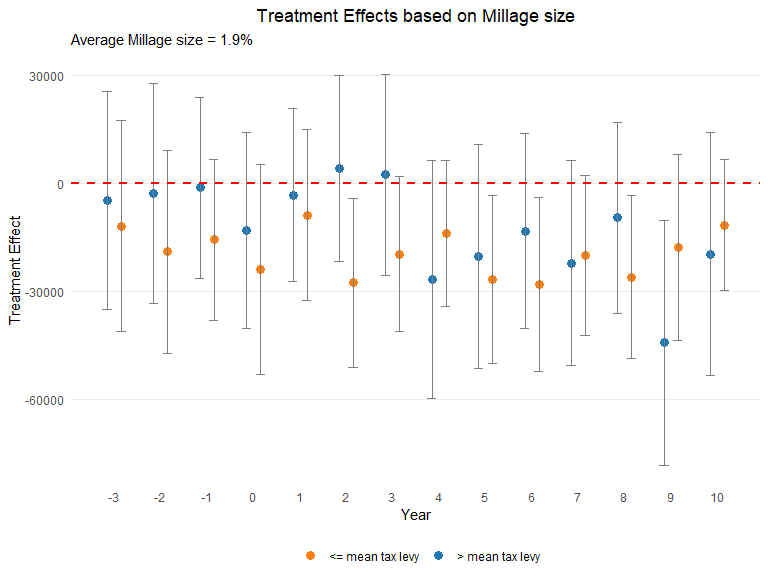
\includegraphics[width=\textwidth,keepaspectratio]{images/tes_size.png}
    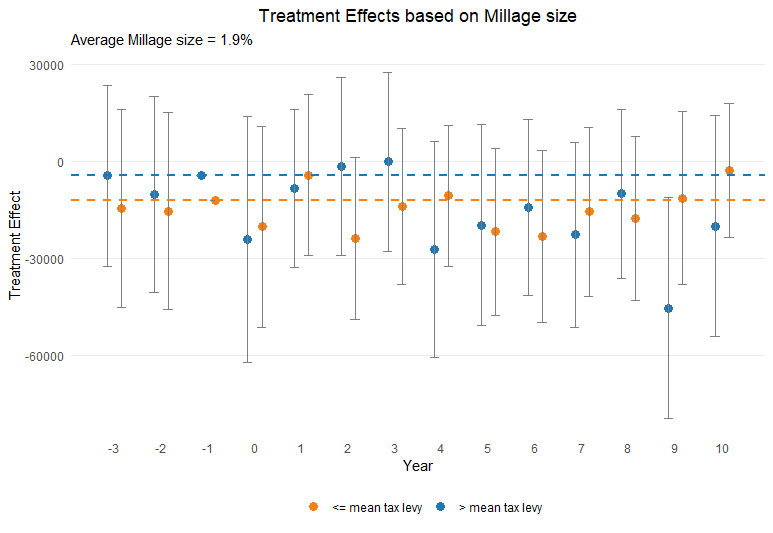
\includegraphics[width=\textwidth,keepaspectratio]{images/tes_size_re.png}    
    \caption{Median Housing Price based on Millage size}
    \label{fig:tes_covs_size}
\end{figure}

All the years before the reduction in road spending have treatment effect estimates with confidence intervals containing zero. Starting in year $t+2$, we observe statistically significant treatment effects in some years after the vote such as year 5, 6 and 8 that show a for tax levies with millage size equal to or below the mean. However, we do not see a consistent decrease in housing prices. Hence, we conclude that the decrease in housing prices of cities that fail to maintain their roads does not vary significantly based on the size of the tax levy.

\vskip 1cm

\textbf{RDD Quantile Estimation}: We further analyze our results by estimating quantile-level treatment effects, as suggested by Frandsen et al (2012), to study how the treatment’s impact varies at different quantiles of the outcome variable. 

\begin{table}[ht]
    \hspace{-1cm}
    % \centering
    \caption{Quantile-level Treatment Effects of Cutting Road Spending on Median House Prices}
    \label{tab:quantile_tes}
    \begin{tabular}{p{1.5cm}ccccccc}
        \hline
        Percentile & $t + 4$ & $t + 5$ & $t + 6$ & $t + 7$ & $t + 8$ & $t + 9$ & $t + 10$ \\
        \hline
        10\% & -6,433 & -22,570 & -9,602 & -12,984 & -11,217 & -6,569 & -1,326 \\
        & (9,364) & (9,065) & (9,205) & (8,420) & (9,136) & (10,809) & (8,793) \\
        20\% & -5,400 & -15,070 & 4,014 & -14,682 & -15,040 & -3,228 & 624 \\
        & (9,983) & (9,886) & (7,443) & (8,502) & (8,160) & (10,435) & (8,509) \\
        70\% & -21,760 & -11,171 & -38,082 & -36,685 & -21,356 & -25,605 & -18,600 \\
        & (12,333) & (11,806) & (12,835) & (12,163) & (12,218) & (13,984) & (9,872) \\
        80\% & -28,478 & -16,379 & -38,460 & -37,470 & -28,950 & -27,800 & -18,658 \\
        & (13,343) & (11,404) & (18,623) & (12,169) & (12,507) & (12,421) & (11,808) \\
        90\% & -51,470 & -34,604 & -38,510 & -27,039 & -29,010 & -49,093 & -36,662 \\
        & (18,409) & (15,837) & (22,194) & (16,308) & (16,640) & (14,498) & (19,110) \\
        \hline
    \end{tabular}
    \begin{tablenotes}
        \small
        \item The outcome is median house price in constant 2010 U.S. dollars. The unit of observation is the city-year, so a treatment effect of -\$28,478 means that at the 80th percentile of house prices four years after the vote, cities that fail to renew road taxes and its associated spending have houses that sell for \$28,478 less than cities that vote to renew road taxes and spending. The regressions include covariates related to the demographics and socioeconomic factors of the cities, drawn from Table \ref{tab:variable_means_sd}.
    \end{tablenotes}
\end{table}

\begin{figure}[htbp]
    \centering
    % 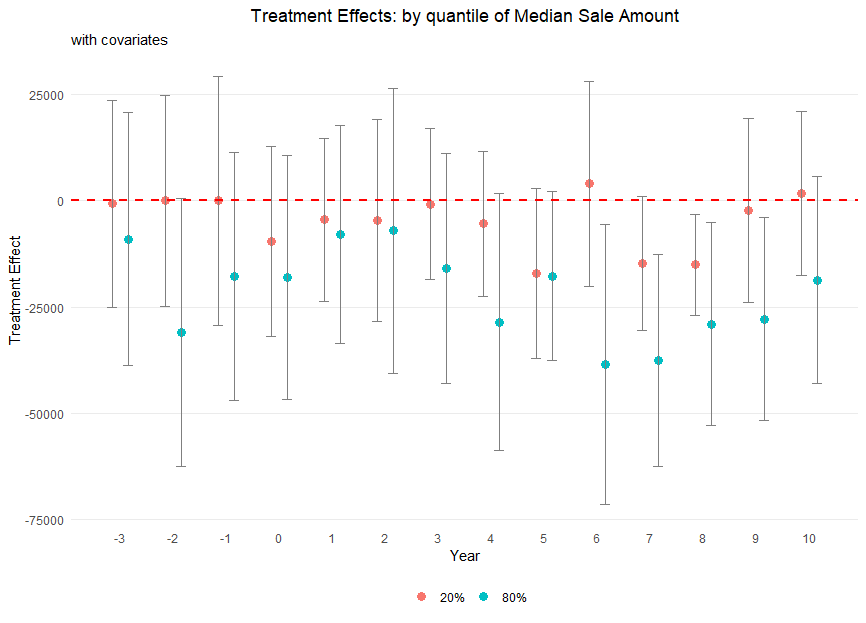
\includegraphics[width=\textwidth,keepaspectratio]{images/tes_qte_covs.png}
    % 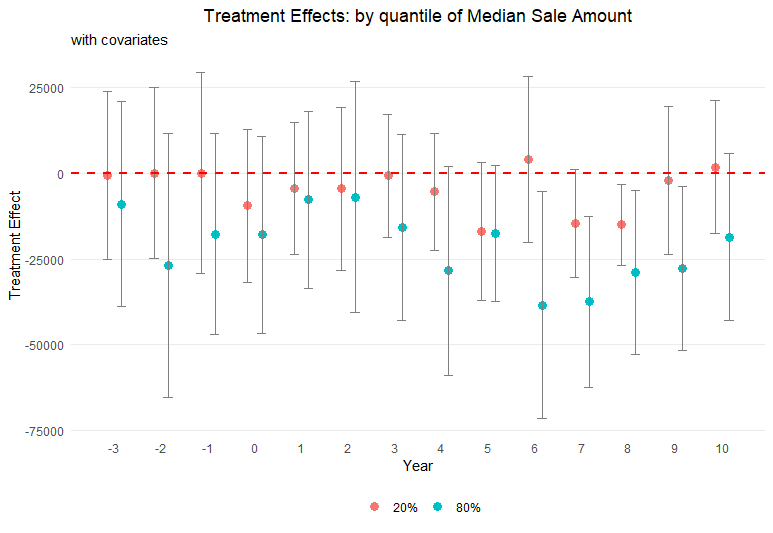
\includegraphics[width=\textwidth,keepaspectratio]{images/tes_qte.png}    
    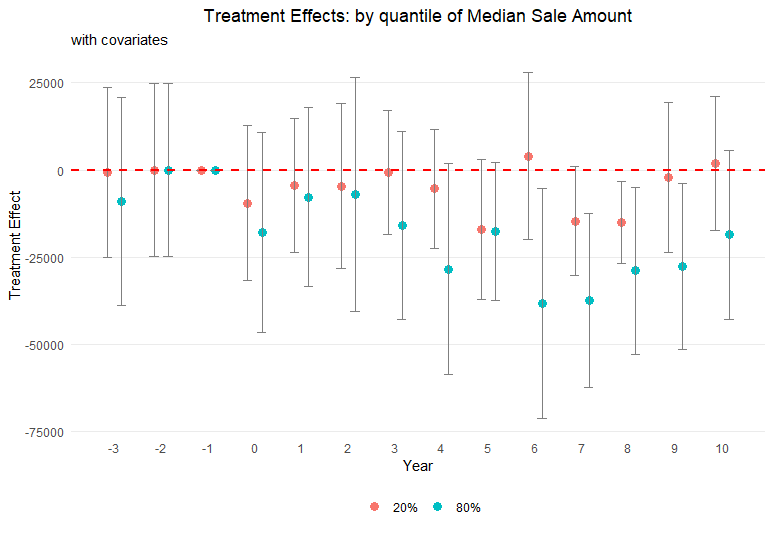
\includegraphics[width=\textwidth,keepaspectratio]{images/tes_qte_re.png}    
    \caption{Median Housing Price based on Quantiles: 20\% and 80\%}
    \label{fig:tes_qte_covs}
\end{figure}

Table \ref{tab:quantile_tes} shows the treatment effect heterogeneity of cutting road spending on high and low quantiles of median house prices. The top percentiles consistently exhibit a statistically significant decline in house sale prices, beginning in year 6 after the reduction in road spending. In contrast, the lower percentiles do not demonstrate a consistent treatment effect. This suggests a differential impact, where higher-valued properties are more sensitive to road disrepair than lower-valued houses. Figure \ref{fig:tes_qte_covs} contrasts the treatment effects of the 20th and 80th percentiles of home sale prices in an effect plot to highlight this differential impact of reduction in road maintenance spending.

\subsection{Robustness Tests}

We conduct several robustness tests to ensure the validity of our results. We test the sensitivity of our results to different bandwidths, covariates, and functional forms. We also check for the presence of pre-trends and perform a placebo test to confirm the validity of our RDD.

\vskip 0.5cm

\textbf{Removing contradictory observations}: In this test, we focus on ensuring the independence and exogeneity of our dataset, a critical aspect in assessing the impact of renewal tax levies on housing prices. An additional concern is the potential bias introduced by tax levies for additional money that might pass after renewal tax levy decisions.
To address this concern, we exclude observations from our analysis if a tax levy for additional funding is introduced and passed within a ten-year period following a renewal tax levy vote. This approach is premised on the notion that the introduction of new funding through additional levies could confound the effects of decreased road taxes on housing prices. 
For example, consider a scenario where a city votes on a renewal tax levy in the year 2000. If that city subsequently introduces and passes a tax levy for additional road spending in 2004, we exclude all votes for that city from 2005 through 2010. This exclusion ensures that the effect on house prices from the 2000 vote are captured for uncontaminated years but not for years after 2004 when the effect of additional road taxes may counteract the drop in tax money from the year 2000 vote. It allows us to isolate and examine the pure impact of the drop in funding from failing renewal levies on housing prices. 

\begin{table}[ht]
    \centering
    \caption{Effect on Median Sale Amount of Failing to Renew a Road Tax Levy}
    \label{tab:uncontaminated}
    \begin{tabular}{p{2.8cm}ccccccc}
        \hline
        year relative to vote & $t + 4$ & $t + 5$ & $t + 6$ & $t + 7$ & $t + 8$ & $t + 9$ & $t + 10$ \\
        \hline
        Treatment effect & -19,015 & -15,609 & -18,403 & -20,842 & -18,950 & -28,634 & -23,823 \\
        standard error   & (9,563) & (10,283) & (10,246) & (9,629) & (9,179) & (7,770)  & (10,594) \\
        Effective bandwidth (h) & 6.88 & 5.92 & 8.36 & 9.42 & 7.91 & 5.43 & 7.05 \\
        Bias bandwidth (b)      & 12.14 & 15.94 & 14.53 & 17.87 & 15.24 & 11.90 & 17.33 \\
        Effective Observations  & 475 & 389 & 561 & 611 & 475 & 300 & 374 \\
        Total Observations      & 2,389 & 2,274 & 2,145 & 2,016 & 1,890 & 1,787 & 1,666 \\
        \hline
    \end{tabular}
    \begin{tablenotes}
        \small
        \item The outcome is median house price in constant 2010 U.S. dollars. The unit of observation is the city-year, so a treatment effect of -\$19,015 means that four years after the vote, cities that fail to renew road taxes and its associated spending have houses that sell for \$19,015 less than cities that vote to renew road taxes and spending. The regressions include covariates related to the demographics and socioeconomic factors of the cities, drawn from Table~\ref{tab:variable_means_sd}.
    \end{tablenotes}
\end{table}


Upon implementing this data filtration, we observe that the treatment effect of the renewal levies on housing prices, measured from $t+1$ to $t+10$, remains largely consistent with our initial findings. This consistency in treatment effect, despite the exclusion of potentially confounding data, lends further credence to our results. The standard errors increase slightly due to reduction in sample size caused by the aforementioned data filtration process. 

\textbf{Placebo cutoffs}: In our primary analysis, the pivotal threshold for the vote share running variable is 50\%, indicating whether a renewal levy passes or fails.  Although we find significant treatment effects using this 50\% threshold, it could be random jumps in the data rather than cutting road taxes and funding that are responsible for the significant estimates.  To this end we conduct a series of placebo tests using alternative cutoffs: 30\%, 40\%, 60\%, and 70\%. Table \ref{tab:placebo_cutoffs} below summarizes the results from the placebo cutoffs analysis. 

\begin{table}[ht]
    \centering
    \caption{Robust Treatment Effect Estimate for Placebo Cutoffs}
    \label{tab:placebo_cutoffs}
    \begin{tabular}{p{2cm}cccc}
        \hline
        Years after vote & 30\% & 40\% & 60\% & 70\% \\
        \hline
        $t + 4$ & 2,578 & 9,149 & 9,419 & -12,987 \\
                & (8,209) & (7,284) & (11,462) & (14,365) \\
        $t + 5$ & -6,381 & -29,077 & 6,383 & 41,683 \\
                & (9,086) & (20,680) & (10,786) & (17,836) \\
        $t + 6$ & 7,681 & 5,573 & -1,095 & -14,226 \\
                & (9,616) & (8,120) & (8,612) & (15,733) \\
        $t + 7$ & 1,162 & 3,982 & -12,050 & 22,261 \\
                & (10,468) & (8,191) & (9,396) & (19,765) \\
        $t + 8$ & 4,334 & 12,881 & 3,593 & 31,696 \\
                & (9,670) & (8,625) & (10,061) & (6,902) \\
        $t + 9$ & 851 & 7,381 & -6,935 & 42,790 \\
                & (5,921) & (6,333) & (7,114) & (15,663) \\
        $t + 10$ & 10,032 & -35,038 & 324 & -8,566 \\
                 & (10,599) & (35,569) & (8,220) & (17,281) \\
        \hline
    \end{tabular}
    \begin{tablenotes}
        \small
        \item Robust treatment effect estimate for placebo cutoffs as per the estimator from \cite{calonico2017rdrobust}. The unit of observation is city-year level. Standard errors are shown in parentheses below each estimate.
    \end{tablenotes}
\end{table}


Table \ref{tab:placebo_cutoffs} does not show consistently significant treatment effects for any of the placebo cutoffs for our parameter of interest. This absence of significance at thresholds other than the true 50\% reinforces the idea that the effects we observe at the 50\% mark are not a mere coincidence or a result of random variation in the data, but are indeed attributable to the dynamics surrounding the passing or failing of renewal tax levies. 

\textbf{Winsorization}: The debate over whether to include or exclude outliers continues, with some research suggesting that trimming outliers does not improve mean squared error (e.g., Bollinger and Chandra, 2005).  We now drop the 1\% tails to help curtail the influence of outliers. The overall sample mean after dropping 1\% tails is \$144,268 in constant 2010 dollars with a standard deviation of \$109,624. After performing this winsorization step, we re-estimate the treatment effect of failing to renew a road tax levy on housing outcome variables. The results from this estimation process are summarized in Figure \ref{fig:tes_g_w} below:

\begin{figure}[htbp]
    \centering
    % 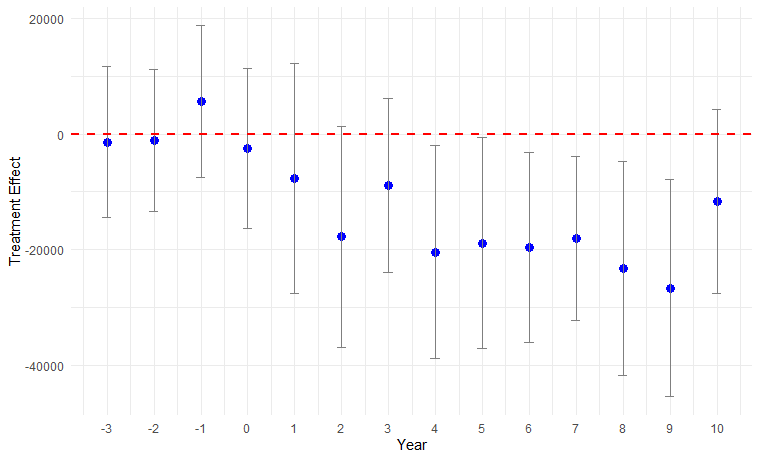
\includegraphics[width=\textwidth,keepaspectratio]{images/tes_g_w.png}
    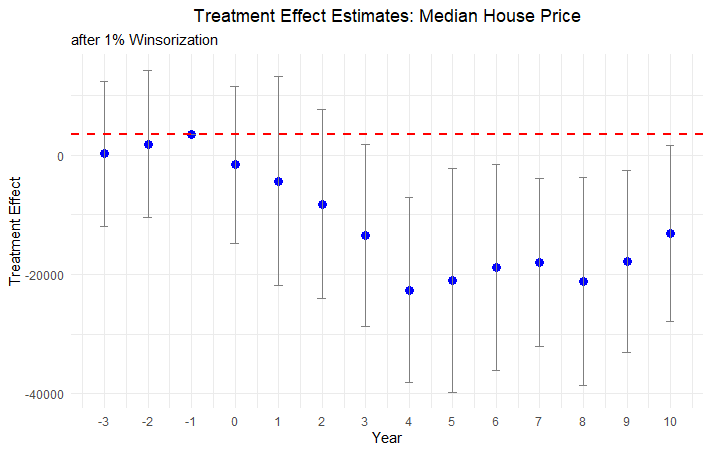
\includegraphics[width=\textwidth,keepaspectratio]{images/tes_g_w_reg.png}    
    \caption{Median Housing Price after 1\% Winsorization}
    \label{fig:tes_g_w}
\end{figure}

The treatment effect estimates with winsorization mimic those from our baseline regression results qualitatively and quantitatively.

\section{Mechanisms} \label{sec:mech}

A key question surrounding our findings is \textit{why} cutting road taxes would lead to a sustained decline in local house prices. In this section, we argue that these results are consistent with classical insights from the literature on local public finance, especially the work of \cite{Tiebout1956} and \cite{Oates1972}. Specifically, cutting road-maintenance tax levies reduces local government funds, which in turn constrains the government’s ability to provide road-upkeep services. This deterioration in road quality then directly and indirectly lowers housing values. Three interconnected channels explain this relationship.

{\bf Road Tax Cuts and Reduced Road Maintenance Funds.} Local governments in Ohio, like those in many other U.S. states, rely on property taxes and dedicated road levies to fund local public goods. The \cite{Oates1972} decentralization theorem highlights that local authorities can generally provide public services in a manner better aligned with resident preferences than would a higher-level government, provided they have adequate revenue sources. When a renewal levy fails at the ballot box, one of these critical revenue sources vanishes. Consistent with the premise that local road quality is a “local public good,” losing a dedicated revenue stream substantially weakens a city’s ability to maintain or upgrade roads. Empirically, we estimate the size of the drop in maintenance funds available to local governments (see Section \ref{sec:data}). In the spirit of \cite{Tiebout1956}, local residents effectively “vote” on their tax and expenditure bundles, which results in a budgetary contraction. Absent compensating resources from state or federal authorities, the lower tax revenue directly reduces spending on maintenance, with ripple effects for local roads and infrastructures.

{\bf Declining Road Quality.} Larger budget constraints produce measurable degradation in road quality. Results from our AI model-based road-quality measure in Section \ref{sec:road_quality_decline} show a marked decrease in road quality following the cessation of renewal levies. The resulting deterioration in road quality may be accompanied by ride discomfort, declining aesthetics, and reduced usability of neighborhood roads. This is precisely what a local public goods framework would predict: fewer financial resources for upkeep immediately impact the daily “consumption” of roads. Residents observe these changes slowly over time, often after four to five years, before road conditions become visibly poor.

{\bf Capitalization into house Prices.} Falling road quality imposes a disamenity on local residents. As recognized by \cite{Oates1969}, property values in a community incorporate expectations of both the level of taxation and the quality of local services. While homebuyers benefit from understanding they might pay lower property taxes in a municipality with a failing levy, they also factor in the anticipated (and eventually realized) deterioration of roads. Several mechanisms help explain the ultimate discount in property values:

\begin{enumerate}
    \item \textbf{Appearance and Neighborhood Appeal.} Rough roads, potholes, and poorly patched surfaces reduce aesthetic appeal. Potential buyers, seeing visible signs of neglect, bid less.
    \item \textbf{Vehicle Damage and Travel Costs.} Chronic maintenance problems translate into higher expenditures on tires, suspensions, and alignments, as well as more time lost to slower commutes.
    \item \textbf{Expectation of Reduced Public Services.} A failed renewal levy may signal broader fiscal stringency, causing residents to expect other future service cutbacks. Uncertainty about service levels weighs negatively on property values. 
\end{enumerate}

\noindent In this sense, the local “bundling” of taxes and roads is priced into real estate transactions, echoing the original proposition of \cite{Tiebout1956} that local public goods are \emph{capitalized} in property values. Our event-study evidence confirms that the negative price effects are most pronounced several years after the renewal levy fails, consistent with the time needed for visible road quality decline to become salient to homeowners and prospective buyers.

{\bf Short-Run versus Long-Run Trade-Off.} Importantly, a trade-off emerges over time. In the short run, residents who voted down the road tax levy experience immediate relief in terms of lower property tax bills. Their out-of-pocket expenses decline, which can be a tangible financial benefit—particularly in communities where property tax burdens were already viewed as high. However, as road quality starts to visibly deteriorate from around the fourth year onward, the same residents find themselves negatively affected by a decline in house prices. This lag reflects the time it takes for infrastructure disrepair to become apparent, be it through more frequent potholes or visibly eroding surfaces. By the time these problems are indisputable, the neighborhood’s real-estate market has had sufficient time to register the disamenity, capitalizing it as a discount in property values. This dynamic captures a fundamental insight of local public finance: the preferences of current taxpayers can diverge from the longer-term public interest \citep{BuchananTullock1962, AlesinaTabellini1990}. While voters may respond to short-term cost savings from a failing levy, the forgone maintenance ultimately reduces the community’s appeal and leads to diminished investment returns—particularly for homeowners whose largest asset is their property. Hence, the immediate reduction in tax liabilities ultimately collides with the reality of lower market valuations once inadequate road upkeep becomes plainly visible.

% \bigskip

In summary, our findings align with longstanding theories of local public finance. Under the logic proposed by \cite{Oates1972}, letting local jurisdictions decide on road tax levies can promote efficient provision of local services, as long as there is sufficient willingness among residents to sustain the quality of road infrastructure. However, once communities choose (either inadvertently or intentionally) to forgo a renewal levy, the immediate reduction in funds and subsequent lagged deterioration in road quality erode property values. From the household’s perspective, subpar road maintenance becomes an undesirable aspect of the local package they are effectively “purchasing” when buying a home, leading to a downward shift in housing demand—and hence, in equilibrium sale prices.

% \section{Mechanisms} \label{sec:mech}

% The central finding of our paper is that local governments experiencing road-tax renewal failures see significant declines in road quality and, subsequently, in housing prices. This section outlines the channels driving this result and connects each to seminal works in infrastructure economics, property valuation, and public finance. Specifically, we discuss: (i) the loss of dedicated revenue streams following failed levies, (ii) the consequent under-provision of road maintenance and deterioration in road quality, and (iii) how poor road quality translates to lower home prices through both functional and perceptual channels.

% \subsection*{1. Reduced Revenue and Under-Provision of Road Maintenance}

% A robust body of literature links infrastructure spending to local economic well-being. \cite{Gramlich1994} underscores how local infrastructure—particularly roads—directly contributes to both residential welfare and business productivity. Once renewal levies fail, municipalities face immediate budgetary shocks, losing earmarked resources for critical repairs and upkeep. Without a guaranteed funding stream, local officials must divert or reduce spending on maintenance and preventative work, creating cumulative disinvestment in road quality over time.

% Budget constraints in local governance often manifest as under-provision of public goods \citep{Fischel2001}, as policymakers are compelled to reallocate limited resources toward other essential services (e.g., law enforcement or general administration). In practice, road maintenance often succumbs to a “defer and patch” strategy that prioritizes urgent fixes at the expense of comprehensive resurfacing projects—resulting in highly visible, steadily worsening road quality.

% \subsection*{2. Physical and Perceptual Decline in Road Quality}

% The deterioration that follows reduced funding is rarely instantaneous; roads degrade gradually, as evidenced by our event-study results. Several scholars note that local infrastructure’s physical depreciation can be slow at first but accelerates without timely maintenance \citep{HoltzEakin1993, Haughwout2002}. In the context of roads, delayed repairs lead to potholes, structural cracks, and uneven surfaces—conditions that, if not remedied, compound into more significant damage requiring costlier interventions down the road.

% Beyond the purely physical aspects, visible degradation fosters negative perceptions of the area among residents and potential homebuyers. The “Homevoter Hypothesis” \citep{Fischel2001} suggests that homeowners, motivated by protecting their property values, closely monitor local government decisions on infrastructure. When they observe (or anticipate) reduced road upkeep, perceptions of overall municipal performance suffer. The resulting belief that road quality will continue to decline can further depress local demand for housing, intensifying the price discount we observe.

% \subsection*{3. Channels Linking Poor Road Quality to Lower Housing Prices}

% \paragraph{(a) Hedonic Valuations.}
% Drawing on the hedonic pricing framework popularized by \cite{Rosen1974}, property values reflect not just the structural characteristics of a home but also neighborhood amenities and disamenities. Deteriorating roads represent a disamenity for multiple reasons: rough driving surfaces impose higher vehicle maintenance costs, commuting is more stressful, and “curb appeal” declines. These factors systematically lower households’ willingness to pay.

% \paragraph{(b) Capitalized Costs and Risks.}
% Local property values incorporate expectations about future taxes and service quality. When road repairs lag, future homeowners anticipate having to pay for tire damage or extra car maintenance, or facing the risk of new, ad-hoc taxation to address infrastructure crises. Such factors become “capitalized” in the purchase price \citep{Brueckner1982}, effectively lowering home valuations if roads are perceived to be underfunded long-term.

% \paragraph{(c) Spatial Externalities and Commuting Costs.}
% Infrastructure scholars such as \cite{HoltzEakin1993} and \cite{Henderson1985} emphasize how higher commuting costs—both monetary and time—reduce the net economic and social benefits of living in certain locations. Poorly maintained local roads amplify these commuting costs, creating a spatial externality that depresses housing demand in neighborhoods where households are likely to endure extra delays or auto-repair expenses.

% \subsection*{Putting It All Together}

% Taken as a whole, these findings present a consistent narrative:
% \begin{enumerate}
%     \item \textbf{Failed levies reduce dedicated funds}, forcing municipalities to cut back on road upkeep or shift limited resources to only the most dire repair tasks.
%     \item \textbf{Road quality gradually declines}, becoming salient to both current and prospective residents, who witness an accumulation of infrastructure problems over multiple years.
%     \item \textbf{Housing prices adjust downward} to reflect new expectations regarding the area’s long-run road conditions, vehicle upkeep costs, and the diminished overall attractiveness of the neighborhood.
% \end{enumerate}

% Importantly, there is a trade-off in the timing of these costs and benefits. In the short run, many residents see an immediate decrease in their out-of-pocket tax expenses when a renewal levy fails. However, as road quality visibly deteriorates over the following years, the longer-term consequence is a decline in neighborhood desirability and thus a drop in house values. This pattern aligns with our empirical finding of significant negative effects on property prices emerging four to five years after a failed road levy vote.

% The lagged effect in house-price reductions aligns with a slower physical manifestation of infrastructure neglect—first, roads appear slightly worn, but only after multiple seasons of continued disinvestment do they exhibit chronic issues that clearly register to prospective homeowners. Buyers and sellers factor these accumulating signals into their transactions, producing the persistent price discount observable several years after the levy failure.

% \bigskip

% In sum, once a road-maintenance levy fails, the structural decline in local infrastructure—both physical and perceptual—becomes a local disamenity capitalized into home values. Seminal scholarship on infrastructure economics and hedonic pricing helps frame how lower road quality translates into reduced property demand, confirming our empirical findings.

\section{Conclusion} \label{sec:conclusion}

A great deal of existing research has focused on the effect of new roads on house prices, especially in developing nations, providing valuable policy insights and spurring development initiatives like China’s Belt \citep{huang2016understanding} and Road Initiative and India’s Pradhan Mantri Gram Sadak Yojana \citep{asher2020}. However, the endogeneity of road placement makes it difficult to identify causal effects. In this paper, we study taxes that fund maintenance of existing roads and avoid endogeneity issues by utilizing a quasi-experiment setting that naturally arises from the voted levies enacted by local governments in Ohio. We study more than 3,000 referendums raised by cities, villages, and townships to renew local road taxes funding existing roads and use dynamic regression discontinuity design to estimate the effect of failure to renew a levy on housing prices. We also estimate the decline in spending experienced by local governments when they face a tax cut due to failure of a renewal tax levy and fine-tune a Vision Transformer model to predict and identify the changes in road quality in these areas. We find an average decline of 17\% in road quality in areas that cut their renewal taxes and a decline in home sale price of 9\% over the 10-year period. We find no anticipation effects, unlike \cite{beenstock2016hedonic} and \cite{diao2017spatial}, but we find statistically significant effects starting four years and continuing onto the later years. We find these effects to be more consistent for urban rather than rural areas. We find a lack of dose-response based on the size of the levy, but we find larger house price reductions for more expensive houses than for cheaper houses.  

\noindent Future research could extend the regression discontinuity identification strategy we employ to other geographies, using vote share as a running variable for places that vote on road spending, or using time as a running variable for cities that directly change road spending without a referendum. Moreover, it could also shift away from studying votes to maintain spending toward studying votes to increase road spending, although the endogeneity of choosing when to propose such a referendum makes identification for such settings more challenging.


